 % - IPC Functionality
 %  - Minimum required per subnet
 %    - Withdrawal/Deposits Interfaces
 %    - Other Operations? (Propagate?)
 %  - Enhancements
 %    - Checkpointing interfaces
 %    - Propagate
 %    - Reporting/Slashing interfaces
 %    - Atomic execution/swap, IBC-like bridges
 %  - Future stuff (google docs?)
 %    - Withdrawal at ancestor (skip parent(s)) (with timeout) etc.
\section{IPC functionality}
\label{sec:functionality}
We list in this section the functionality that should be provided by the IPC components. We first list the minimal functionality required for every subnet (deposits and withdrawals), to then extend it with enhanced functionalities. We model components as processes that produce and consume events. Events consumed by the IPC agent are the result of either a notification from one of the SMRs or the response of a query made by the IPC agent. Events produced by the IPC agent result in the IPC agent submitting a transaction that will change the state of the SMR that consumes the event.

We note that our focus is on the core functionalities, disregarding optimizations for the moment. Batching is a prime example of this. It is expected that batching will be a key optimization whenever \verifyGfinal{\tx}{\prf} is used, as calling \verifyGfinal{\tx}{\prf} can be costly. Batching allows us to perform multiple operations for one \verifyGfinal{\tx}{\prf} call, reducing its overall cost.

\subsection{Minimal Functionality}
\label{sec:minFunc}
We show in this section the functionalities for deposits and withdrawals.

\subsubsection{Deposits}
\label{sec:deposit}

\arp{Consider need to pause/remedy subnet after deposit (e.g. collateral not enough with new supply). IPC agent should check in that case}\\

A deposit is a transfer of funds (of some amount \fil) from user $\user_P$'s wallet in the parent subnet to user $u_C$'s wallet in the child subnet.
We assume that $u_P$ is a participant running a parent replica, a child replica, and an \ipc agent.%
\footnote{If $u_P$ does not run these processes, $u_P$ contacts a trusted participant that does and that performs the deposit on $u_P$'s behalf.}
The deposit is performed by the user controlling the \ipc agent as follows:
\begin{enumerate}
    \item The local \ipc agent submits to the parent \smr replica the corresponding (properly signed) transaction
    $\tx=\textit{Deposit}\left( \src, \fil, \sa.\textit{accounts}.\dest \right)$ with $\src=\user_P$ and $\dest = \user_C$.
    \item The parent SMR system orders and executes the Deposit transaction (provided $u_P$ has enough funds) by transferring $amt$ from $u_P$'s parent account to the \sa (concretely, to $u_P$'s account representation within the \sa). This effectively locks the funds within the \sa \dapp, until the \sa \dapp transfers it back to $u_P$'s account during withdrawal (see \Cref{sec:withdraw}).
    \item When the parent's replicated state that includes the transaction becomes final (for some SMR-system-specific definition of finality), the local parent replica notifies the local \ipc agent, potentially attaching a proof of finality of $PoF(tx)$ to the notification.%
    \footnote{The exact content of $PoF(tx)$ depends on the implementations of the SMR systems. It might contain, for example, a quorum of replica signatures, a Merkle proof of inclusion, or even be empty.}
    \item The \ipc agent constructs a transaction $\tx' = \textit{Deposited}\left(\langle  \src, \fil, \sa.\textit{accounts}.\dest \rangle, \prf \right)$ and submits it to the child SMR system.
    \item Upon ordering $tx'$, the replicated logic of the child SMR system mints \fil new coins and adds them to $\user_C$'s account.
\end{enumerate}

We show in \Cref{fig:deposit} the events being produced and consumed by the deposit functionality and in Algorithm~\ref{alg:deposit} the pseudocode per component to implement the functionality.

\begin{figure}[h]
     \centering
     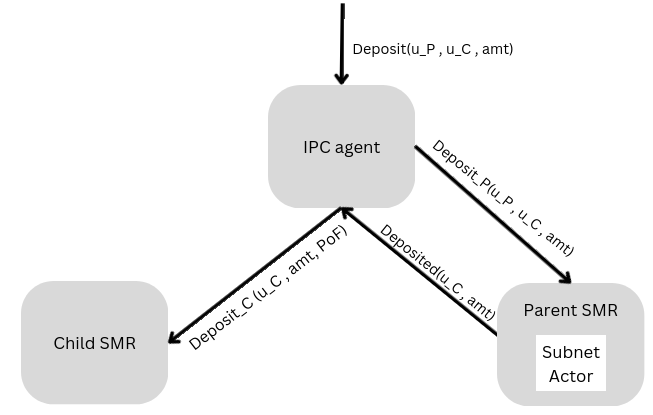
\includegraphics[width=\textwidth]{deposit}
     \caption{Events produced and consumed during a deposit.}
     \label{fig:deposit}
\end{figure}
 

\begin{algorithm}[H]
\footnotesize
\caption{Deposit operation}\label{alg:deposit}
  \DontPrintSemicolon
  \SetKwFunction{FMain}{Global}
  \SetKwProg{Pn}{Function}{:}{\KwRet}
  \SetKwInOut{Input}{input}
  \SetKwProg{Component}{$\blacktriangleright$ \bf}{:}{\KwRet}
  \SetKwFor{UponKW}{upon}{do}{fintq}
  \Input{\src account in parent, \dest account in child, amount~$\fil$}
   \Component{IPC agent}{
        submit $\tx=\textit{Deposit}\left( \src, \fil, \sa.\textit{accounts}.\dest \right)$ to parent \smr replica\;
  }
   %
   \Component{Parent \smr replica}{
   \UponKW{\tx}{
    move $\fil$ from \src to \sa.\textit{accounts}.\dest  \tcp*[r]{"lock" at parent}
    notify agent \texttt{ParentDeposited}(\tx)
   }
  }
  \Component{IPC agent}{
    \UponKW{notification of \texttt{ParentDeposited}(\tx) from parent \smr}{
        create \prf that \tx is final at parent \smr \tcp*[r]{see Sec.~? for details}
        submit \texttt{Deposited}$=\langle \tx, \prf \rangle$ to child \smr    
     }
  }
  \Component{Child \smr replica}{
    \UponKW{\texttt{Deposited}}{
        assert \prf for \tx\;
        increase \dest account by \fil
     }
  }
\end{algorithm}
One thing that differs a downward transaction (e.g., deposit) from an upward transaction (e.g., checkpoint) is that any participant that operates the child \smr replica also has visibility into the state of the parent \smr (albeit stale) through its local parent \smr replica. This enables the \textbf{local validity check} method to assert the finality at the parent (which may or may not be preferred over others).%
\footnote{\textbf{local validity check} (simpler, efficient, \textit{weaker guarantees}): $\prf$ contains a pointer to the block containing \tx  at the parent, together with the height~$h$ of that block.
 To assert that \tx is final, the child queries the parent about $TX$, if it exists -- return valid, else -- return invalid. If invalid but the parent is still below height~$h$, then query again when parent reaches height~$h$.
This is a test inside the child \smr process. Therefore, if we want this method (and I believe we do), we should widen the interface so that a child \smr can ask the agent to get data from the parent. However, this optimization comes at the expense of the encapsulation of components, that is, it entails tinkering with the child \smr code.}
            
\subsubsection{Withdrawals}
\label{sec:withdraw}

A withdrawal is a transfer of funds from user $u_C$'s wallet in the child subnet to some user $u_P$'s wallet in the parent subnet. We assume that $u_C$ is a participant running a parent replica, a child replica and an \ipc agent. The withdraw is performed as follows:
\begin{enumerate}
  \item $u_C$ triggers the $Withdraw(u_C, u_P, amt)$ event at the local \ipc agent.
    \item The local \ipc agent submits the corresponding (properly signed) transaction $tx = Withdraw_C(u_C, u_P, amt)$ to the child SMR system.
    \item The child SMR system orders and executes the Withdraw transaction, burning $amt$ funds in $u_C$'s account (provided $u_C$ has enough funds).
    \item When the child's replicated state that includes the transaction becomes final (for some SMR-system-specific definition of finality that has been defined in the SA), the local child replica notifies the local \ipc agent, potentially attaching a proof \prf that this state is final.%
    \item The \ipc agent constructs a transaction $tx' = Burned(u_P, amt, \prf)$ and submits it to the parent SMR system.
    \item Upon ordering $tx'$, the replicated logic of the parent SMR system updates the state of the SA transferring the funds from \sa (concretely, to $u_P$'s account representation within the \sa) to $u_P$'s account.
\end{enumerate}

 \begin{figure}[h]
     \centering
     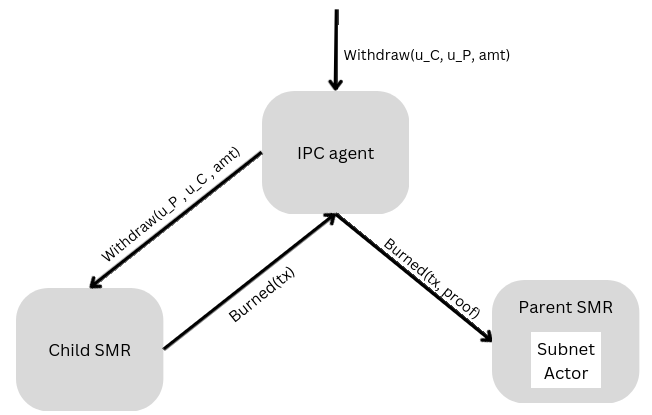
\includegraphics[width=\textwidth]{withdrawal}
     \caption{Events produced and consumed during a withdrawal.}
     \label{fig:withdrawal}
 \end{figure}
\begin{algorithm}[H]
\footnotesize
\caption{Withdraw operation}\label{alg:down}
  \DontPrintSemicolon
  \SetKwFunction{FMain}{Global}
  \SetKwProg{Pn}{Function}{:}{\KwRet}
  \SetKwInOut{Input}{input}
  \SetKwProg{Component}{$\blacktriangleright$ \bf}{:}{\KwRet}
  \SetKwFor{UponKW}{upon}{do}{fintq}
  % \Input{user~$\user$, amount~$\fil$, transaction \txnf}
   \Input{\src account in child, \dest account in parent, $\fil$ amount of coins}
   \Component{IPC agent}{
        submit $\tx=\textit{Withdraw}(\src, \fil, \dest)$ to child \smr\;
  }
   %
   \Component{Child \smr replica}{
   \UponKW{$\tx = \textit{Withdraw}(\src, \fil, \dest)$}{
    deduct $\fil$ from \src account at child \tcp{``burns" \fil in child}
    notify agent \texttt{Burned}(\tx)
   }
  }
  \Component{IPC agent}{
    \UponKW{notification of \texttt{Burned}(\tx) from child \smr replica}{
    
        create \prf that \tx is final at child \smr \tcp*[r]{see Sec.~? for details}
        submit $\tx'=\texttt{Burned}\left(\tx, \prf \right)$  to parent \smr replica
     }
  }
  \Component{parent \smr replica}{
    \UponKW{$\tx'=\texttt{Burned}\left(\tx, \prf \right)$}{
        assert \sa.\verifyGfinal{\prf}{\tx}\;
        move \fil coins from \sa.accounts[\src] to \dest
     }
  }
   
%    \Component{Child SMR}{
%    [\tx submitted by user, proposed, written]\\
%    \UponKW{\txnf written in Child SMR}{
%     decrease user fund's by $\fil$\\
%     Send \texttt{ChildWithdrawn(\tx, [$proof$])} to IPC agent \tcp*[r]{notify IPC agent}
%    }
%   }
%   \Component{IPC agent}{
%     \UponKW{\texttt{ChildWithdrawn(\tx, [$proof$])} notified by Child SMR}{
%     \If{$proof=$ \textbf{nil}}{
%          $proof \gets $\textit{generateProofOfGlobalFinality(\tx,...)} \tcp*[r]{Necessary steps for \tx to be ready to be submitted to Parent SMR}
%      }
%      \texttt{ChildWithdrawn(\tx, $proof$)} to parent SMR \tcp*[r]{Submit to parent}
%      }
%     \UponKW{\arp{State updated after Withdrawal}}{ \tcp*[r]{Notified when parents update state}
%       \arp{Check child subnet rules are still satisfied, remedy/close otherwise?}
%     }
%   }
%   \Component{Parent SMR}{
%   \UponKW{\texttt{ChildWithdrawn(\tx, $proof$)} submitted by IPC agent}{
%       \If{\sa.\verifyGfinal{\tx}{\prf}}{
%            [tx submitted by IPC agent, proposed, written]\\
%            \UponKW{\txnf written in Parent SMR}{
%                 reduce $\fil$ amount for user $\user$ in SA\\
%                 Parent SMR notifies IPC agent
%             }
%       }
%   }
% }
\end{algorithm}
\subsection{Enhanced Functionality}
We show here a list of desirable functionalities that build upon the basic withdrawals and deposits.
\subsubsection{Checkpointing} A checkpoint contains a representation of the updated state of the child SMR system to be included in the parent SMR system. A checkpoint can be triggered by predefined events (i.e. periodically after a number of state updates, triggered by a specific user or set of users, etc.). As such, the checkpoint functionality may or may not be triggered by a user request on the child SMR. A checkpoint is performed as follows: 
\begin{enumerate}
\item If the predefined checkpoint trigger is met, then the IPC agent queries the child SMR replica for the updated state to be represented in this checkpoint.
\item The IPC agent creates a proof \prf that this updated state of the child SMR system is final, possibly compressing its representation of the state.
\item The IPC agent submits a transaction $\tx'=\texttt{Checkpoint}\left(\textit{state}, \prf \right)$ to the parent SMR replica
 \item Upon ordering $tx'$, the replicated logic of the parent SMR system updates the state of the SA according to the checkpoint state, if necessary.
\end{enumerate}

\begin{figure}[h]
     \centering
     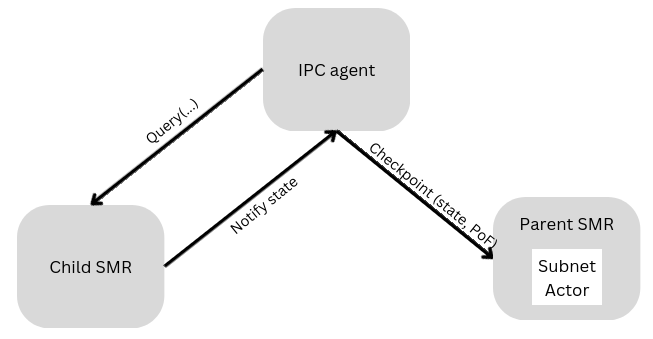
\includegraphics[width=\textwidth]{checkpoint.png}
     \caption{Events produced and consumed by the checkpointing functionality.}
     \label{fig:chkp}
 \end{figure}
\begin{algorithm}[H]
\footnotesize
\caption{Checkpoint operation}\label{alg:down}
  \DontPrintSemicolon
  \SetKwFunction{FMain}{Global}
  \SetKwProg{Pn}{Function}{:}{\KwRet}
  \SetKwInOut{Input}{input}
  \SetKwProg{Component}{$\blacktriangleright$ \bf}{:}{\KwRet}
  \SetKwFor{UponKW}{upon}{do}{fintq}
   \Component{IPC agent}{
        \If{trigger for checkpoint}{
            \textit{state} $\gets$ query the child \smr replica for the state\;
            create \prf that \textit{state} is final at child \tcp*[r]{Possibly compress \textit{state}}
        }
        submit $\tx'=\texttt{Checkpoint}\left(\textit{state}, \prf \right)$  to parent \smr replica
  }
  \Component{parent \smr replica}{
    \UponKW{$\tx'=\texttt{Checkpoint}\left(\textit{state}, \prf \right)$}{
        assert \sa.\verifyGfinal{\prf}{\textit{state}}\;
        $\sa.\textit{latestCheckpoint} \gets \textit{state}$
     }
  }
  
  % \Input{[User's checkpoint request]}
  % \Component{Child SMR}{
  %    \UponKW{State updated [ \textbar User's checkpoint request]}{ 
  %       [Write checkpoint request if any]\\
  %      Send \texttt{StateUpdated($st$)} to IPC agent \tcp*[r]{Notify IPC agent}
  %    }
  % }
  % \Component{IPC agent}{
  %   \UponKW{\texttt{StateUpdated($st$)} notified by child SMR}{
  %       \If{\texttt{SatisfiesCheckpointCondition($st$)}}{
  %          Create checkpoint \chkp\\
  %           $proof \gets $\textit{generateProofOfGlobalFinality($st$,...)} \tcp*[r]{Necessary steps for \tx to be ready to be submitted to Parent SMR}
  %           Submit \texttt{SubmitCheckpoint(\chkp)} to parent SMR
  %           }
  %       }
  % }
  % \Component{Parent SMR}{
  %     \UponKW{\texttt{SubmitCheckpoint(\chkp)} submitted by IPC agent}{
  %        [\chkp proposed, written]\\
  %        Refund fee to submitter \tcp*[r]{refund at parent for simplicity}
  %     }
  % }
\end{algorithm}

\subsubsection{Slashing} 
\guy{This section is immature for review (even a preliminary one)}\\
We show here the events produced and consumed by the slashing functionality. Given specific misbehavior from participants that is identified as Proofs of Fraud (PoFs), e.g.
gathering signed equivocating messages, the child SMR reports the PoFs to the IPC agent, which immediately forwards a slash a request to the parent SMR. \arp{Extend with need to verify if child SMR can continue, needs to remedy its depleted collateral or should be killed with latest checkpoint/state update}.
\begin{figure}[h]
     \centering
     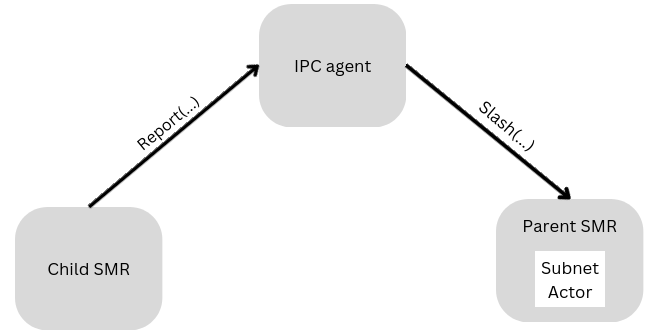
\includegraphics[width=\textwidth]{slash}
     \caption{Events produced and consumed by the slashing functionality.}
     \label{fig:report}
 \end{figure}\\

\begin{algorithm}[H]
\footnotesize
\caption{Slash Functionality}\label{alg:down}
  \DontPrintSemicolon
  \SetKwFunction{FMain}{Global}
  \SetKwProg{Pn}{Function}{:}{\KwRet}
  \SetKwInOut{Input}{input}
  \SetKwProg{Component}{$\blacktriangleright$ \bf}{:}{\KwRet}
  \SetKwFor{UponKW}{upon}{do}{fintq}
  \Input{-}
  \Component{Child SMR}{
     \UponKW{Proofs of fraud \pofs generated}{
       Notify \report to IPC agent
     }
  }
  \Component{IPC agent}{
    \UponKW{\report notified by child SMR}{
        Submit \slashop to parent SMR
    }
    \UponKW{\arp{State updated after slashing}}{
      \arp{Check child SMR rules are still satisfied, remedy/close otherwise?}
    }
  }
  \Component{Parent SMR}{
        \UponKW{\slashop submitted by IPC agent}{
         Update SA state slashing/excluding participants
         Notify SA update to IPC agent
        }
  }
\end{algorithm}


\subsubsection{\postoffice}
The \postoffice functionality is an inter-subnet transaction service. The main motivation for this functionality comes from a ``potential clients" request: enable a \dapp in one subnet to interact with a \dapp in a different subnet.\\
\guy{Edge case: a leaf subnet does not have a \sa and, therefore, no \postoffice. We can consider removing the \postoffice functionality from the \sa and to deploy it as an independent \dapp that will appear only once per subnet. In this case, it needs permissions to call \sa.\verifyGfinal{\tx}{\prf} function.}

\begin{algorithm}[H]
\footnotesize
\caption{\postoffice Functionality}\label{alg:po}
  \DontPrintSemicolon
  \SetKwFunction{FPropagate}{propagate}
  \SetKwProg{Pn}{Function}{:}{\KwRet}
  \SetKwInOut{Input}{input}
  \SetKwProg{Component}{$\blacktriangleright$ \bf}{:}{\KwRet}
  \SetKwProg{Empty}{\bf}{:}{\KwRet}
  \SetKwFor{UponKW}{upon}{do}{fintq}
  \Input{$\tx = \langle \data, \src, \dest, \prf \rangle$}
  \Component{\sa.\postoffice}{
     \UponKW{\postoffice.\propagate(\tx) }{
       \Case{\dest in current subnet}{
            \postoffice.\propagate\textit{HERE}(\tx)
       }
       \Case{\dest requires going up the tree}{
            \postoffice.\propagate\textit{UP}(\tx)
       }
       \Case{\dest requires going down the tree}{
            \postoffice.\propagate\textit{DOWN}(\tx)
       }
     }
     \UponKW{\postoffice.\propagate\textit{UP}(\tx) }{
       \If{\src not from this subnet}{
            assert(\sa.\verifyGfinal{\tx}{\prf})\;
       }
       \src.\textit{append(\sa's subnet id)}\;
       emit event \postoffice.UP$\langle \data, \src, \dest \rangle$
     }
     \tcp{\propagate\textit{DOWN}(\tx) is analogous to \propagate\textit{UP}(\tx)}
     \tcp{\propagate\textit{HERE}(\tx) is trivial}
  }
  \Component{parent \smr process}{
     \UponKW{event \postoffice.UP$\langle \data, \src, \dest \rangle$}{
        $\tx \gets \langle \data, \src, \dest \rangle$\;
        notify agent on \postoffice.UP(\tx)
     }
  }
  \Component{IPC agent}{
    \UponKW{notification of \propagate\textit{UP}(\tx) from child \smr}{
        create \prf that \textit{UP}(\tx) is final at child \smr\;
        $\tx_\textit{new}\gets\langle \textit{UP}(\tx), \prf \rangle$\;
        submit \sa.\postoffice.\propagate($\tx_\textit{new}$) to parent \smr
    }   
}
\end{algorithm}
\subsubsection{Atomic Execution}
TODO Discuss in Lanzarote?
\label{enhancedFunc}

\subsection{Future}
\label{sec:future}